%%%%%%%%%%%%%%%%%%%%%%%%%%%%%%%%%%%%%%%%%
% Stylish Article
% LaTeX Template
% Version 2.1 (1/10/15)
%
% This template has been downloaded from:
% http://www.LaTeXTemplates.com
%
% Original author:
% Mathias Legrand (legrand.mathias@gmail.com) 
% With extensive modifications by:
% Vel (vel@latextemplates.com)
%
% Authors:
% Mauricio Hoyos Ardila mhoyosa2@eafit.edu.co
% Jonathan Zapata Castaño jzapat80@eafit.edu.co
%
% License:
% CC BY-NC-SA 3.0 (http://creativecommons.org/licenses/by-nc-sa/3.0/)
%
%%%%%%%%%%%%%%%%%%%%%%%%%%%%%%%%%%%%%%%%%

%----------------------------------------------------------------------------------------
%	PACKAGES AND OTHER DOCUMENT CONFIGURATIONS
%----------------------------------------------------------------------------------------

\documentclass[fleqn,10pt]{SelfArx} % Document font size and equations flushed left

\usepackage[english]{babel} % Specify a different language here - english by default

\usepackage{lipsum} % Required to insert dummy text. To be removed otherwise

%----------------------------------------------------------------------------------------
%	COLUMNS
%----------------------------------------------------------------------------------------

\setlength{\columnsep}{0.55cm} % Distance between the two columns of text
\setlength{\fboxrule}{0.75pt} % Width of the border around the abstract

%----------------------------------------------------------------------------------------
%	COLORS
%----------------------------------------------------------------------------------------

\definecolor{color1}{RGB}{0,0,0} % Color of the article title and sections
\definecolor{color2}{RGB}{0,20,20} % Color of the boxes behind the abstract and headings

%----------------------------------------------------------------------------------------
%	HYPERLINKS
%----------------------------------------------------------------------------------------

\usepackage{hyperref} % Required for hyperlinks
\hypersetup{hidelinks,colorlinks,breaklinks=true,urlcolor=color2,citecolor=color1,linkcolor=color1,bookmarksopen=false,pdftitle={Title},pdfauthor={Author}}

%----------------------------------------------------------------------------------------
%	ARTICLE INFORMATION
%----------------------------------------------------------------------------------------

\JournalInfo{Reporte Técnico, No. 1, 2017} % Journal information
\Archive{Universidad EAFIT} % Additional notes (e.g. copyright, DOI, review/research article)

\PaperTitle{Clústering de Documentos a partir de Métricas de Similitud} % Article title

\Authors{Mauricio Hoyos\textsuperscript{1}, Jonathan Zapata\textsuperscript{2}} % Authors
\affiliation{\textsuperscript{1}\textit{Departamento de Ingeniería de Sistemas, Universidad EAFIT, Medellín, Colombia, } \textbf{mhoyosa2@eafit.edu.co}} % Author affiliation
\affiliation{\textsuperscript{2}\textit{Departamento de Ingeniería de Sistemas, Universidad EAFIT, Medellín, Colombia, } \textbf{jzapat80@eafit.edu.co}} % Author affiliation

\Keywords{K-means --- Jacard --- MPI --- Cluster --- HPC --- Paralelización --- Particionamiento por dominio --- Similitud } % Keywords 

\newcommand{\keywordname}{Keywords} % Defines the keywords heading name

%----------------------------------------------------------------------------------------
%	ABSTRACT
%----------------------------------------------------------------------------------------

\Abstract{Text mining is an analysis technique which has allowed us to implement a set of new applications through the time. Such as search engines in the web (Google, Facebook, Amazon, Spotify, Netflix, among others), suggestions systems, natural language processing and others.
The document clustering techniques enable us to link a document with other similar documents according to a comparison metric.
The basic idea of the proposed implementations is to compare the efficiency between computing in a single node and computing in a distributed network of nodes.}

%----------------------------------------------------------------------------------------

\begin{document}

\flushbottom % Makes all text pages the same height

\maketitle % Print the title and abstract box

\tableofcontents % Print the contents section

\thispagestyle{empty} % Removes page numbering from the first page

%----------------------------------------------------------------------------------------
%	ARTICLE CONTENTS
%----------------------------------------------------------------------------------------

\section*{Introducción} % The \section*{} command stops section numbering

\addcontentsline{toc}{section}{Introducción} % Adds this section to the table of contents

Actualmente, debido a la gran cantidad de información que se encuentra en los medios, y a que está alojada en diferentes bases de datos, surge la necesidad de agrupar dicha información en un conjunto de datos que permita realizar búsquedas más rápidas, para ello se  crearon técnicas que permiten calcular la similitud que tienen dos textos; una de las más utilizadas es la minería de datos, la cual, como su nombre lo indica, se encarga de extraer las partes importantes de un archivo (en nuestro caso un texto). El enfoque que le dimos al proyecto está delimitado precisamente por esta área de la ciencia de datos, la cual nos va a permitir crear varios set de documentos y determinar el número de sets apropiados para agrupar la información, esto gracias a diferentes experimentos, además de generar un informe detallado evaluando el contraste (figura \ref{fig:graficoSerialParalelo},\ref{fig:graficoParaleloAceleracion}) de compartamientos entre el tiempo de ejecución del programa en serial y el paralelo con diferentes datasets.

En este caso, decidimos hacer que la agrupación de documentos sea mediante el uso de los algoritmos k-means y Jaccard, estos son el principal soporte para determinar la similitud entre documentos.
 
 
 \begin{figure*}[ht]\centering % Using \begin{figure*} makes the figure take up the entire width of the page
 	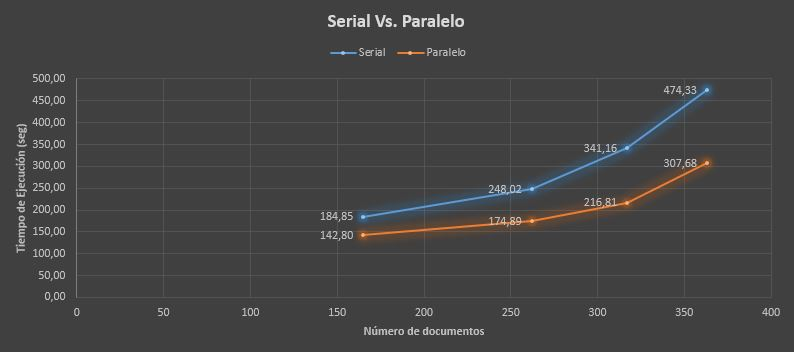
\includegraphics[width=\linewidth]{graficoSerialParalelo}
 	\caption{Gráfico Serial Vs. Paralelo}
 	\label{fig:graficoSerialParalelo}
 \end{figure*}
 
 
 
 \begin{figure*}[ht]\centering % Using \begin{figure*} makes the figure take up the entire width of the page
 	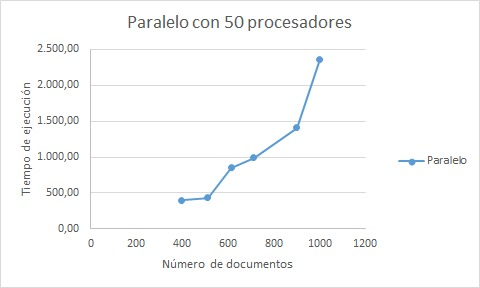
\includegraphics[width=\linewidth]{graficoParaleloAceleracion}
 	\caption{Gráfico Tiempo de Ejecución Vs. Cantidad de documentos}
 	\label{fig:graficoParaleloAceleracion}
 \end{figure*}
%------------------------------------------------

\section{Marco Teórico}


%\begin{enumerate}[noitemsep] % [noitemsep] removes whitespace between the items for a compact look
%\item First item in a list
%\item Second item in a list
%\item Third item in a list
%\end{enumerate}


\begin{description}
	\item[K-means Algorithm] “The k-means method has been shown to be effective in producing good clustering results for many practical applications. However, a direct algorithm of k-means method requires time proportional to the product of number of patterns and number of clusters per iteration. This is computationally very expensive especially for large datasets.
	The number of iterations required can vary in a wide range from a few to several thousand depending on the number of patterns, number of clusters, and the input data distribution. Thus, a direct implementation of the k-means method can be computationally very intensive. This is especially true for typical data mining applications with large number of pattern vectors” \cite{K-means}. 
	
	The algorithm is composed of the following steps:
	Place K points into the space represented by the objects that are being clustered. These points represent initial group centroids.
	
	
	Assign each object to the group that has the closest centroid.
	
	
	When all objects have been assigned, recalculate the positions of the K centroids.
	
	
	Repeat Steps 2 and 3 until the centroids no longer move. This produces a separation of the objects into groups from which the metric to be minimized can be calculated.
	
	figura sacada del mismo paper. \cite{K-means Algorithm}
	The number of K is determinate by the user and indicate the number of clusters.
	
	\item[Jaccard Algorithm] 
	“This is a particular notion of ‘similarity’: the similarity of sets by looking at the relative size of their intersection.
	The Jaccard similarity of sets S and T is |S instersected T |/|S union T |, that is, the ratio of the size of the intersection of S and T to the size of their union. We shall denote the Jaccard similarity of S and T by SIM(S, T ).  An important class of problems that Jaccard similarity addresses well is that of finding textually similar documents in a large corpus such as the Web or a collection of news articles. We should understand that the aspect of similarity we are looking at here is character-level similarity, not “similar meaning,” which requires us to examine the words in the documents and their uses.” \cite{jaccard_similarity}. 
	“To calculate the Jaccard dissimilarity the Jaccard similarity matrix is computed first and thereafter transformed.”\cite{jaccard_seudo}
	This can be reach following this steps:
	Count the number of members which are shared between both sets.
	Count the total number of members in both sets (shared and un-shared).
	Divide the number of shared members by the total number of members.
	Multiply the number you found in by 100. \cite{jaccard_steps}
	
	\item[Document Clustering] Is the act of collecting similar documents in sets. “Document clustering involves the use of descriptors and descriptor extraction. Descriptors are sets of words that describe the contents within the cluster. Document clustering is generally considered to be a centralized process. Examples of document clustering include web document clustering for search users.
	A web search engine often returns thousands of pages in response to a broad query, making it difficult for users to browse or to identify relevant information. Clustering methods can be used to automatically group the retrieved documents into a list of meaningful categories, as is achieved by e.g. open source software such as Carrot2.
	” \cite{document clustering}
	“Agglomerative hierarchical clustering and K-means are two clustering techniques that are commonly used for document clustering. Agglomerative hierarchical clustering is often portrayed as 'better' than K-means, although slower. “ \cite{Doc_clust_techniques}
	
	\item[HPC] 
	"High-performance computing (HPC) is the use of parallel processing for running advanced application programs efficiently, reliably and quickly. The term applies especially to systems that function above a teraflop or 1012 floating-point operations per second. The term HPC is occasionally used as a synonym for supercomputing, although technically a supercomputer is a system that performs at or near the currently highest operational rate for computers. Some supercomputers work at more than a petaflop or 1015 floating-point operations per second.” \cite{hpc_def} This includes “using the world's fastest and largest computers to solve large problems.” \cite{parallel_comp_lawrence_nat_lab}
	“High Performance Computing most generally refers to the practice of aggregating computing power in a way that delivers much higher performance than one could get out of a typical desktop computer or workstation in order to solve large problems in science, engineering, or business.” \cite{hpc}
	
	\item[Parallel computing] 
	Is a technique that consists of execute many calculations at the same time to solve big problems in less time than it could take in conventional computing. There are different kinds of parallel computing:
	“Instruction-level parallelism (ILP): Multiple instructions from the same instruction stream can be executed concurrently this kind is limited in practice by data and control dependences.
	Thread-level or task-level parallelism (TLP): Multiple threads or instruction sequences from the same application can be executed at the same time those could be generated by compiler/user and managed by compiler and hardware and is limited in practice by communication/synchronization overheads and by algorithm characteristics.
	Data-level parallelism (DLP): Instructions from a single stream operate concurrently on several data is limited by non-regular data manipulation patterns and by memory bandwidth 
	Transaction-level parallelism: Multiple threads/processes from different transactions can be executed concurrently and is limited by concurrency overheads”\cite{Parallel Computing}.
	\item[Domain Partition] “In this type of partitioning, the data associated with a problem is decomposed. Each parallel task then works on a portion of the data.” \cite{parallel_comp_lawrence_nat_lab}
	
	\item[MPI] 
	“MPI is a standardized and portable message-passing system. Message-passing systems are used especially on distributed machines with separate memory for executing parallel applications. With this system, each executing process will communicate and share its data with others by sending and receiving messages. MPI is the specification resulting from the MPI-Forum which involved several organizations designing a portable system (that can allow programs to work on a heterogeneous network).
	Since the data can only be shared by exchanging messages, this standard is not intended for use on shared-memory systems, like a multiprocessor computer. Basically, MPI includes point-to-point communication, collective communication (over a network of processes), process groups, bindings for Fortran and C and other advanced functions” \cite{MPI}
	
	\item[MPI Directives]
	Mpi directives are a set of collective communication routines and some variants:
	MPI\_Bcast
	“A broadcast is one of the standard collective communication techniques. During a broadcast, one process sends the same data to all processes in a communicator. One of the main uses of broadcasting is to send out user input to a parallel program, or send out configuration parameters to all processes.” \cite{mpi_bcast}.
	MPI\_Scatter 
	“Is a collective routine that is very similar to MPI\_Bcast. MPI\_Scatterinvolves a designated root process sending data to all processes in a communicator. The primary difference between MPI\_Bcast and MPI\_Scatteris that MPI\_Bcast sends the same piece of data to all processes while MPI\_Scatter sends chunks of an array to different processes.
	MPI\_Gather is the inverse of MPI\_Scatter. Instead of spreading elements from one process to many processes, MPI\_Gather takes elements from many processes and gathers them to one single process. This routine is highly useful to many parallel algorithms, such as parallel sorting and searching” \cite{mpi_directives}.
	
	\item[Overhead (computing)] “The amount of time required to coordinate parallel tasks, as opposed to doing useful work. Parallel overhead can include factors such as:
	- Task start-up time
	- Synchronizations
	- Data communications
	- Software overhead imposed by parallel languages, libraries, operating system, etc.
	- Task termination time”  \cite{parallel_comp_lawrence_nat_lab}
	
	
\end{description}

%\begin{itemize}[noitemsep] % [noitemsep] removes whitespace between the items for a compact look
%	\item First item in a list
%	\item Second item in a list
%	\item Third item in a list
%\end{itemize}

%\subsubsection{Subsubsection}

%------------------------------------------------

\section{Análisis y Diseño (PCAM)}

\paragraph{Particionamiento:}
Esta característica fue tenida en cuenta en el momento de realizar el conteo de palabras ya que cada nodo puede realizarlo sobre un grupo diferente de datos sin depender del conteo de los demás nodos. 
De esta misma manera se emplea el particionamiento al realizar el conteo de las palabras más importantes seleccionadas  mediante los cálculos previos.
Este puede ser considerado un buen particionamiento ya que divide tanto los cálculos asociados con el problema como los datos sobre los cuales opera.

\paragraph{Comunicación:}
El proceso de comunicación es de vital importancia, ya que nos permite obtener los datos que requiere cada nodo para realizar las funciones que le fueron encargadas, esta fase de comunicación se puede evidenciar cuando se hacen operaciones de lectura y escritura de datos que se encuentran en otros nodos, en este caso hace falta la aplicación de dicha técnica.


\paragraph{Aglomeración:}
Los algoritmos empleados para determinar la similitud y comparación de diferentes textos necesita juntar toda la información procesada por los nodos, así que dicha información es aglomerada en un solo nodo para la ejecucion de instrucciones de naturaleza serial, este tipo de fase en la que se recurre a la separación y recolección de datos, es la que más aplicamos en el transcurso de toda la ejecución.

\paragraph{Mapeo:}
La tecnología nos permite fácilmente repartir tareas entre los diferentes nodos, independientemente del número que haya, por lo que garantizamos mapeo al asignar una tarea al número de nodos que le asignamos a la ejecución del programa. Cada tarea es asignada a un procesador, en nuestro caso aplicamos mucho el concepto SIMD.

Los algoritmos que usamos están descritos en el marco teórico, pues son técnicas ampliamente probadas.
Las estructuras de datos que usamos son las fundamentales (int, bool, char[], matrices, etc), diccionarios y listas.
En cuanto al rendimiento análitico de la solución se puede encontrar que es de orden cúbico.

El diseño del algoritmo Jaccard que usamos lo sacamos de este sitio \cite{jaccard_seudo}. 

\section{Implementación}
La implementación de esta practica fue realizada en python ya que es un lenguaje de programación muy sencillo de utilizar pero principalmente por que los modulos de MPI son de facil instalación y utilización.
Para la implementacíon del codigo serial se utilizaron algunas bibliotecas como operator, os y sys que nos permitieron realizar operaciones como lectura de ficheros, manejo de argumentos y brindar caracteristicas para el ordenamiento de alguas estructuras de datos, tambien se empleo numpy como un soporte para las estructuras de datos necesarias para la matriz que contenia todas las distancias entre documentos.
Para la implementación del algoritmo en paralelo se emplearon las librerias anterior mente mencionadas, pero además se empleó la biblioteca mpi4py que es la implementacion de Message Passing Interface para python, dicha biblioteca facilita todo el proceso de mensajeria que se requiere entre nodos para cumplir con el proceso de aglomeración y comunicación.

Es importante recalcar que la implementación del algoritmo en paralelo fue diseñada y desarrollada con el fin de que no se dependiera de una estructura expecifica del hardware y que se pudiera correr dependiendo del nuemero de nodos especificados por el programador/usuario al correrlo. 

A continuación compartimos nuestra implementación alojada en Github, en la cual basamos el análisis presentado en este estudio; al interior de este ling podra encontrar un Readme.md con todas las instrucciones necesarias por poder correr satisfactoriamente los diferentes algoritmos: \href{https://github.com/jonyzp/HPC}{Repositorio de Github}

\section{Análisis de resultados (secuencial vs. paralelo)}

A continuación presentamos el gráfico resultante del proceso de medición, el cual evidencia las aceleraciones entre datasets e implementaciones y en distintas ejecuciones.

\begin{table}[hbt]
	\caption{Tabla de Comparaciones de tiempo}
	\centering
	\begin{tabular}{llr}
%		\toprule
%		\multicolumn{1}{c}{Parámetro de comparación} \\
		\cmidrule(r){1-3}
		SetSize (MB) & T. Serial (seg) & T. Paralelo (seg)\\
		\midrule
		
		119,92 & 474,33 & 307,68 \\
		
		94,88 & 341,16 & 216,81 \\
		
		75,02 & 248,02 & 174,89 \\
		
		68,66 & 184,85 & 142,80 \\
		
		\bottomrule
	\end{tabular}
	\label{tab:label}
\end{table}


Se puede evidenciar la diferencia entre ejecutar el algoritmo de forma paralela a ejecutarlo de manera serial, aunque el algoritmo paralelo tiene un mayor orden de complejidad, logra reducir el tiempo que tarda en dar la solución, ya que el procesamiento se realiza de una manera distribuída




%------------------------------------------------
\phantomsection
\section*{Conclusiones} % The \section*{} command stops section numbering


\begin{itemize}
	\item Hay que saber atacar adecuadamente el problema para identificar qué procesos son los que se pueden optimizar por medio del procesamiento en co-paralelo
	\item Debido al tipo de dato que se estaba manejando en el procesamiento de los nodos es difícil optimizar pensando en la fase de la aglomeración de los datos.
	\item Es de anotar que no siempre se da por sentado que antes de resolver un problema hay que sentarse a diseñar primero, por lo que no sobra mencionar la importancia de tener al lado una hoja y un lápiz.
	\item La manera de estructurar un algoritmo serial comparada con la del paralelo cambia, precisamente para facilitar la paralelización, o en ocasiones, porque representa un limitante de implementación.
\end{itemize}
% So long and thanks for all the fish \cite{Figueredo:2009dg}.

%----------------------------------------------------------------------------------------
%	REFERENCE LIST
%----------------------------------------------------------------------------------------


\begin{thebibliography}{9}

\bibitem{K-means}
Alsabti, K., Ranka, S. and Singh, V. (2017). An Efficient K-Means Clustering Algorithm. [online] pp.1-2. \href{https://www.cs.utexas.edu/~kuipers/readings/Alsabti-hpdm-98.pdf}{Available clicking here} [Accessed 22 Oct. 2017].
\bibitem{K-means Algorithm}
Home.deib.polimi.it. (2017). Clustering - K-means. [online] \href{http://home.deib.polimi.it/matteucc/Clustering/tutorial_html/kmeans.html}{Available clicking here} [Accessed 22 Oct. 2017].


\bibitem{jaccard_seudo}
Schulz, D. (2017). Jaccard similarity. [online] Code10.info. 
\href{http://www.code10.info/index.php?option=com_content&view=article&id=60:articlejaccard-similarity&catid=38:cat_coding_algorithms_data-similarity&Itemid=57}{Available clicking here} [Accessed 22 Oct. 2017].

\bibitem{jaccard_similarity} 

Standford University Infolab. (2017). \textit{Finding Similar Items}. [online] \href{http://infolab.stanford.edu/~ullman/mmds/ch3.pdf}{Available clicking here} [Accessed 22 Oct. 2017].

\bibitem{jaccard_steps} 
Statistics How To. (2017). Jaccard Index / Similarity Coefficient. [online] [Accessed 22 Oct. 2017].
\href{http://www.statisticshowto.com/jaccard-index/}{Available clicking here}  [Accessed 22 Oct. 2017].


\bibitem{document clustering}
En.wikipedia.org. (2017). Document clustering. [online] \href{https://en.wikipedia.org/wiki/Document_clustering}{Available clicking here} [Accessed 22 Oct. 2017].

\bibitem{Doc_clust_techniques} 
Glaros.dtc.umn.edu. (2017). A Comparison of Document Clustering Techniques | Karypis Lab. [online] \href{http://glaros.dtc.umn.edu/gkhome/node/157}{Available clicking here} [Accessed 22 Oct. 2017].

\bibitem{hpc} 
insideHPC. (2017). What is high performance computing? - insideHPC. [online] \href{https://insidehpc.com/hpc-basic-training/what-is-hpc/}{Available clicking here}  [Accessed 22 Oct. 2017].

\bibitem{hpc_def} 
SearchDataCenter. (2017). What is high-performance computing (HPC)? - Definition from WhatIs.com. [online] 
\href{http://searchdatacenter.techtarget.com/definition/high-performance-computing-HPC}{Available clicking here}   [Accessed 22 Oct. 2017].


\bibitem{parallel_comp_lawrence_nat_lab} 
Computing.llnl.gov. (2017). Introduction to Parallel Computing. [online] \href{https://computing.llnl.gov/tutorials/parallel_comp/}{Available clicking here}  [Accessed 22 Oct. 2017].


\bibitem{Parallel Computing}
Types of Parallelism. [online] \href{http://www.inf.ed.ac.uk/teaching/courses/pa/Notes/lecture02-types.pdf}{Available clicking here} [Accessed 22 Oct. 2017].


\bibitem{MPI}
En.wikibooks.org. (2017). Message-Passing Interface - Wikibooks, open books for an open world. [online] \href{https://en.wikibooks.org/wiki/Message-Passing_Interface}{Available clicking here} [Accessed 22 Oct. 2017].

\bibitem{mpi_bcast} 
Mpitutorial.com. (2017). MPI Broadcast and Collective Communication · MPI Tutorial. [online] \href{http://mpitutorial.com/tutorials/mpi-broadcast-and-collective-communication/}{Available clicking here} [Accessed 22 Oct. 2017].

\bibitem{mpi_directives} 
Mpitutorial.com. (2017). MPI Scatter, Gather, and Allgather · MPI Tutorial. [online] \href{
	http://mpitutorial.com/tutorials/mpi-scatter-gather-and-allgather/}{Available clicking here} [Accessed 22 Oct. 2017].

\bibitem{DISENO DE ALGORITMOS PARALELOS}
DISENO DE ALGORITMOS PARALELOS. cs.buap. (2017). [online] \href{https://www.cs.buap.mx/~mtovar/doc/ProgConc/ProgramacionParalela.pdf}{Available clicking here} [Accessed 21 Oct. 2017].

\end{thebibliography}


%----------------------------------------------------------------------------------------


% no BORRAR:
%\begin{verbatim}
%CODE HERE
%\end{verbatim}


\end{document}
